\subsubsection{TENT} \label{sssec:tent}

When this map is implemented in a computer using any numerical representation system (even floating-point!) truncation errors rapidly increase and make unstable fixed point in $x^*=0$ to become stable.
The sequences within the attractor domain of this fixed point will have a short transitory of length between $0$ and $B$ followed by an infinite number of $0$'s \cite{Jessa2002,Callegari}.
This issue is easily explained in \cite{Li2004}, the problem appears because all iterations have a left-shift operation that carries the $0$'s from the right side of the number to the most significant positions.
Some authors \cite{buscar} have proposed to add random perturbations to avoid this drawback of the Tent map.
This procedure improves the statistical properties of the time series, but what really happens is that the statistical properties of the random perturbations are mixed with those of the Tent map.
Here we study the Tent map ``as it is" without any artifice to evaluate its real behaviour, instead of theoretical statistical properties. 

Figs. \ref{fig:TENT_QuantiB} (a) to (e) show the quantifiers for floating- and fixed-point numerical representations.
Quantifiers $H_{hist}$, $H_{BP}$ and $C_{BP}$ are equal to zero for all precisions, this reflects that the series quickly converge toward a fixed point for all sequences.
In the case of $H_{BPW}$ and $C_{BPW}$ quantifiers are different to non-null because BPW procedure discards the elements once they reach the fixed point.
The high dispersions in $H_{BPW}$, $C_{BPW}$ and MP are related to the short length of series transient.
These transients that converge to a fixed point have a maximum length of $B$ iterations for fixed-point arithmetic and $80$ for floating-point (long double precision).

\begin{figure}
	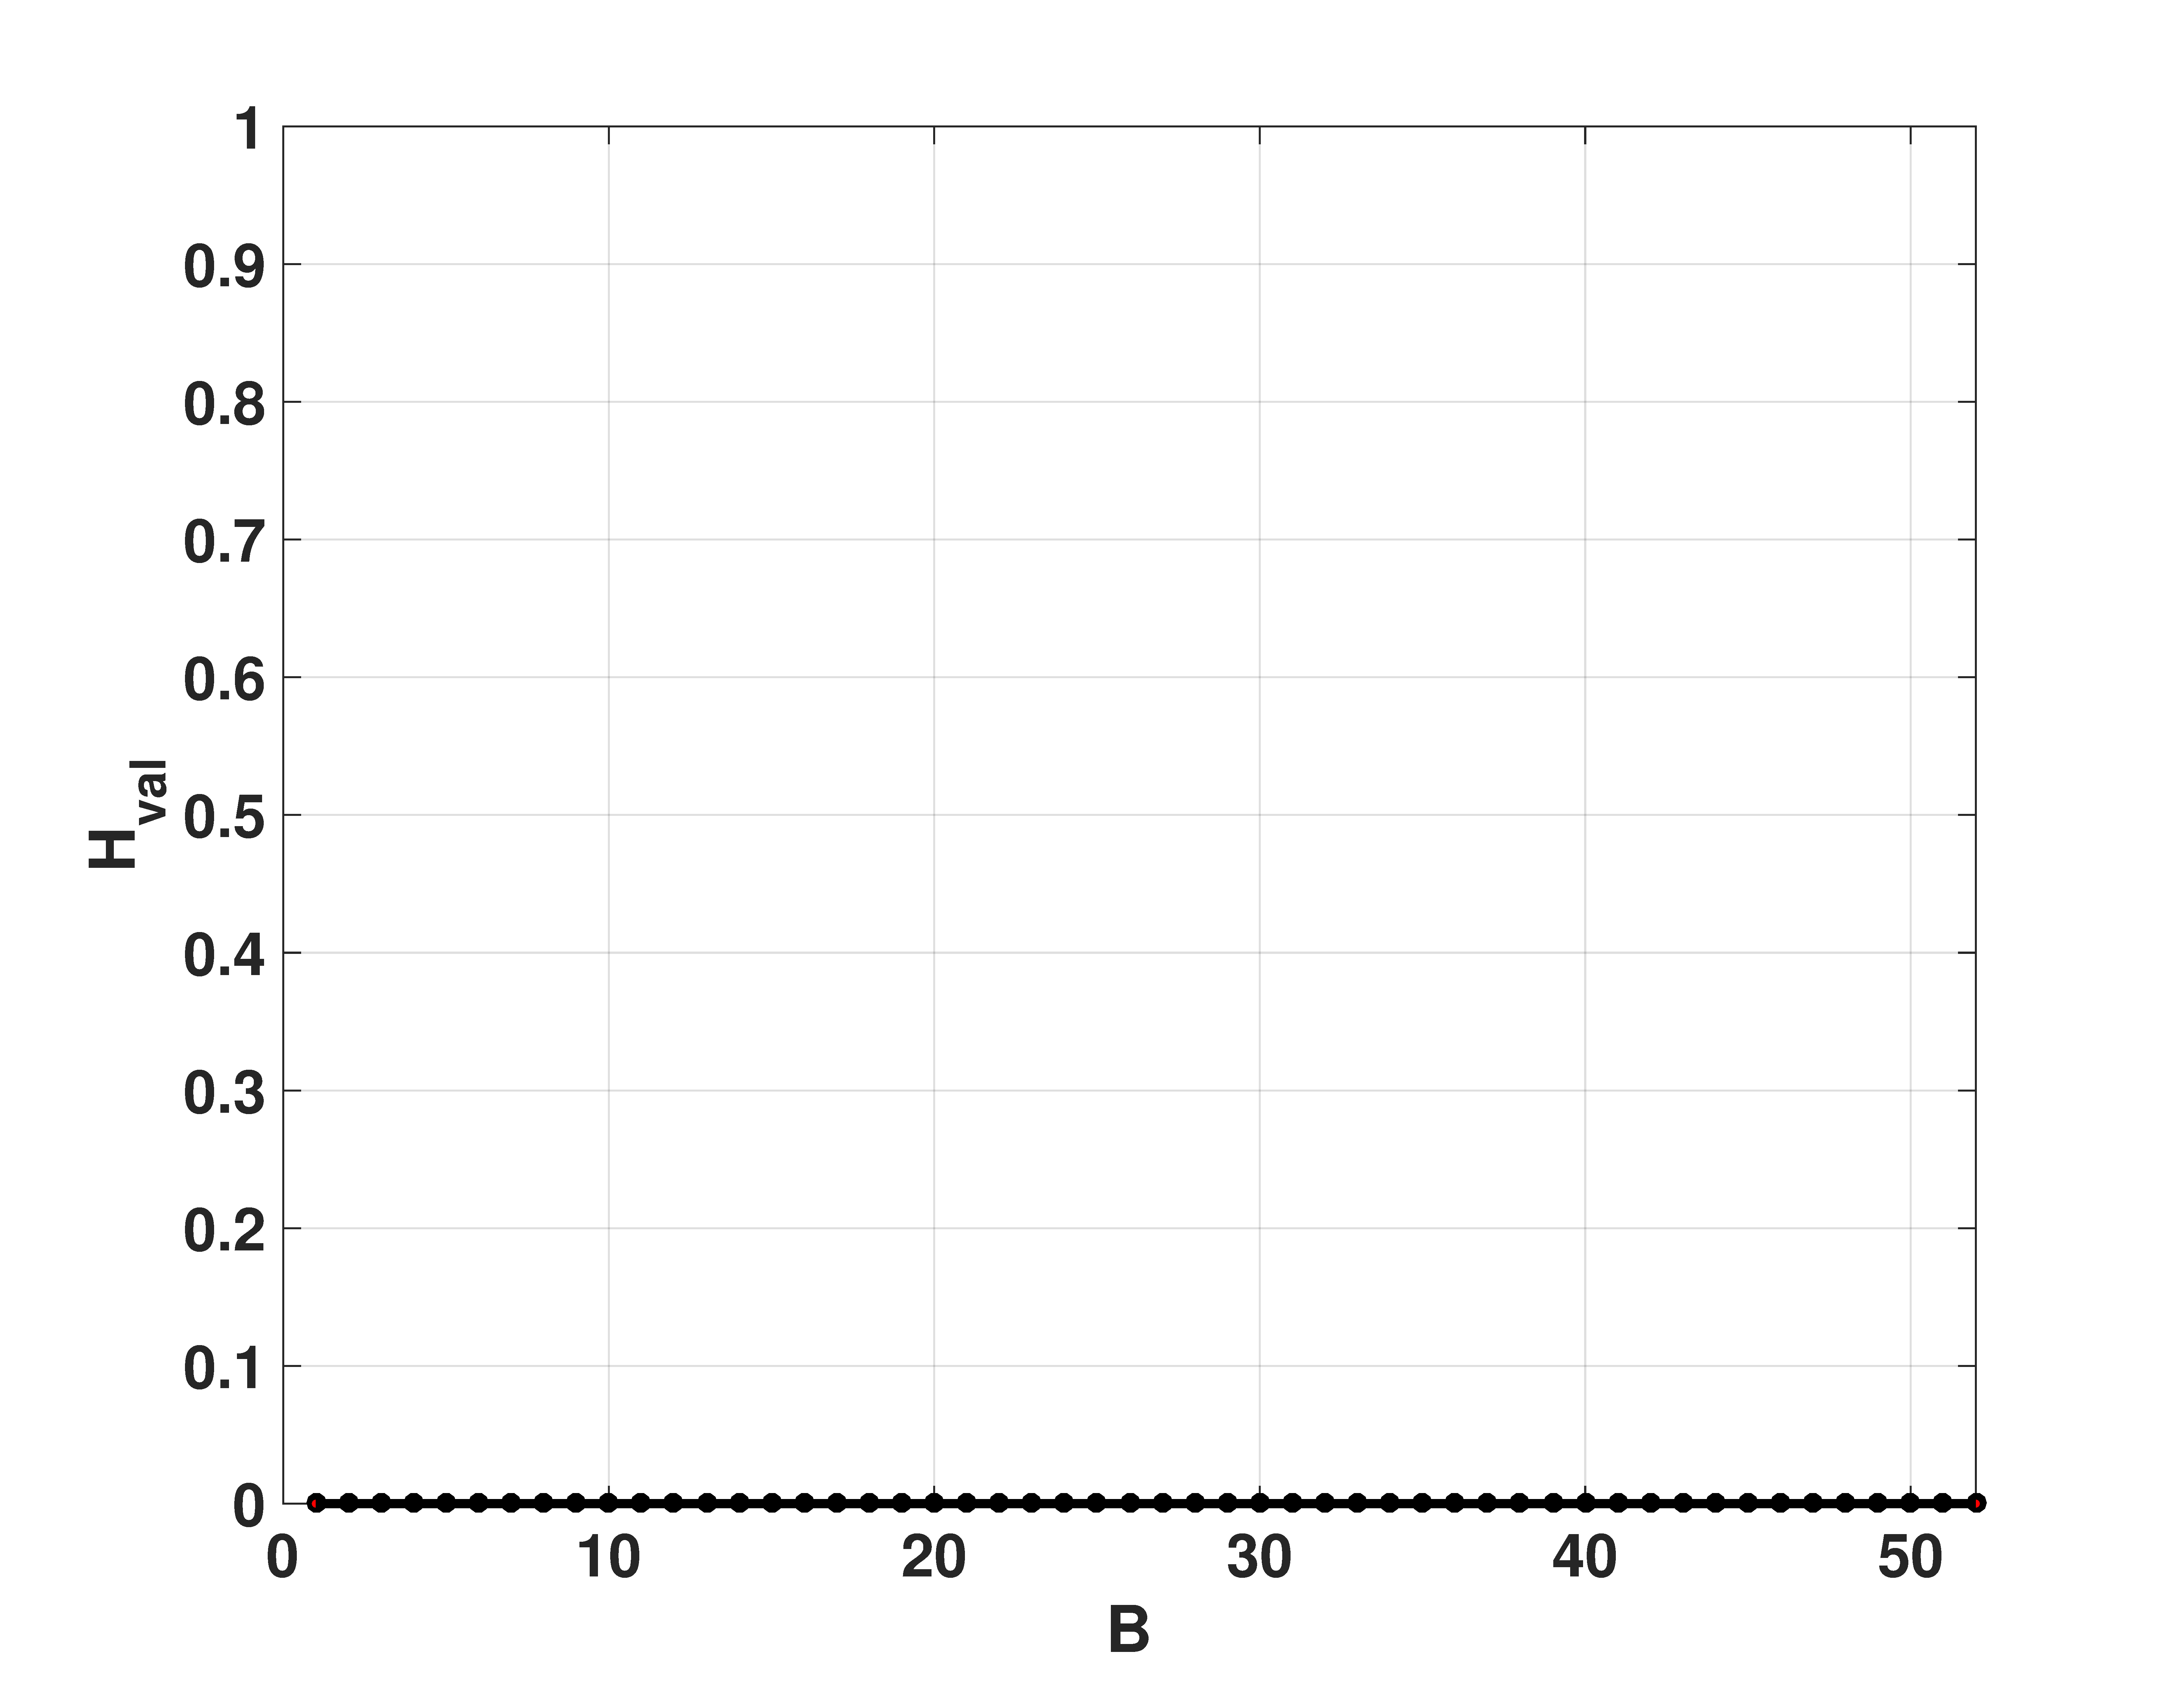
\includegraphics[width=.49\textwidth]{Hval_Tent}
	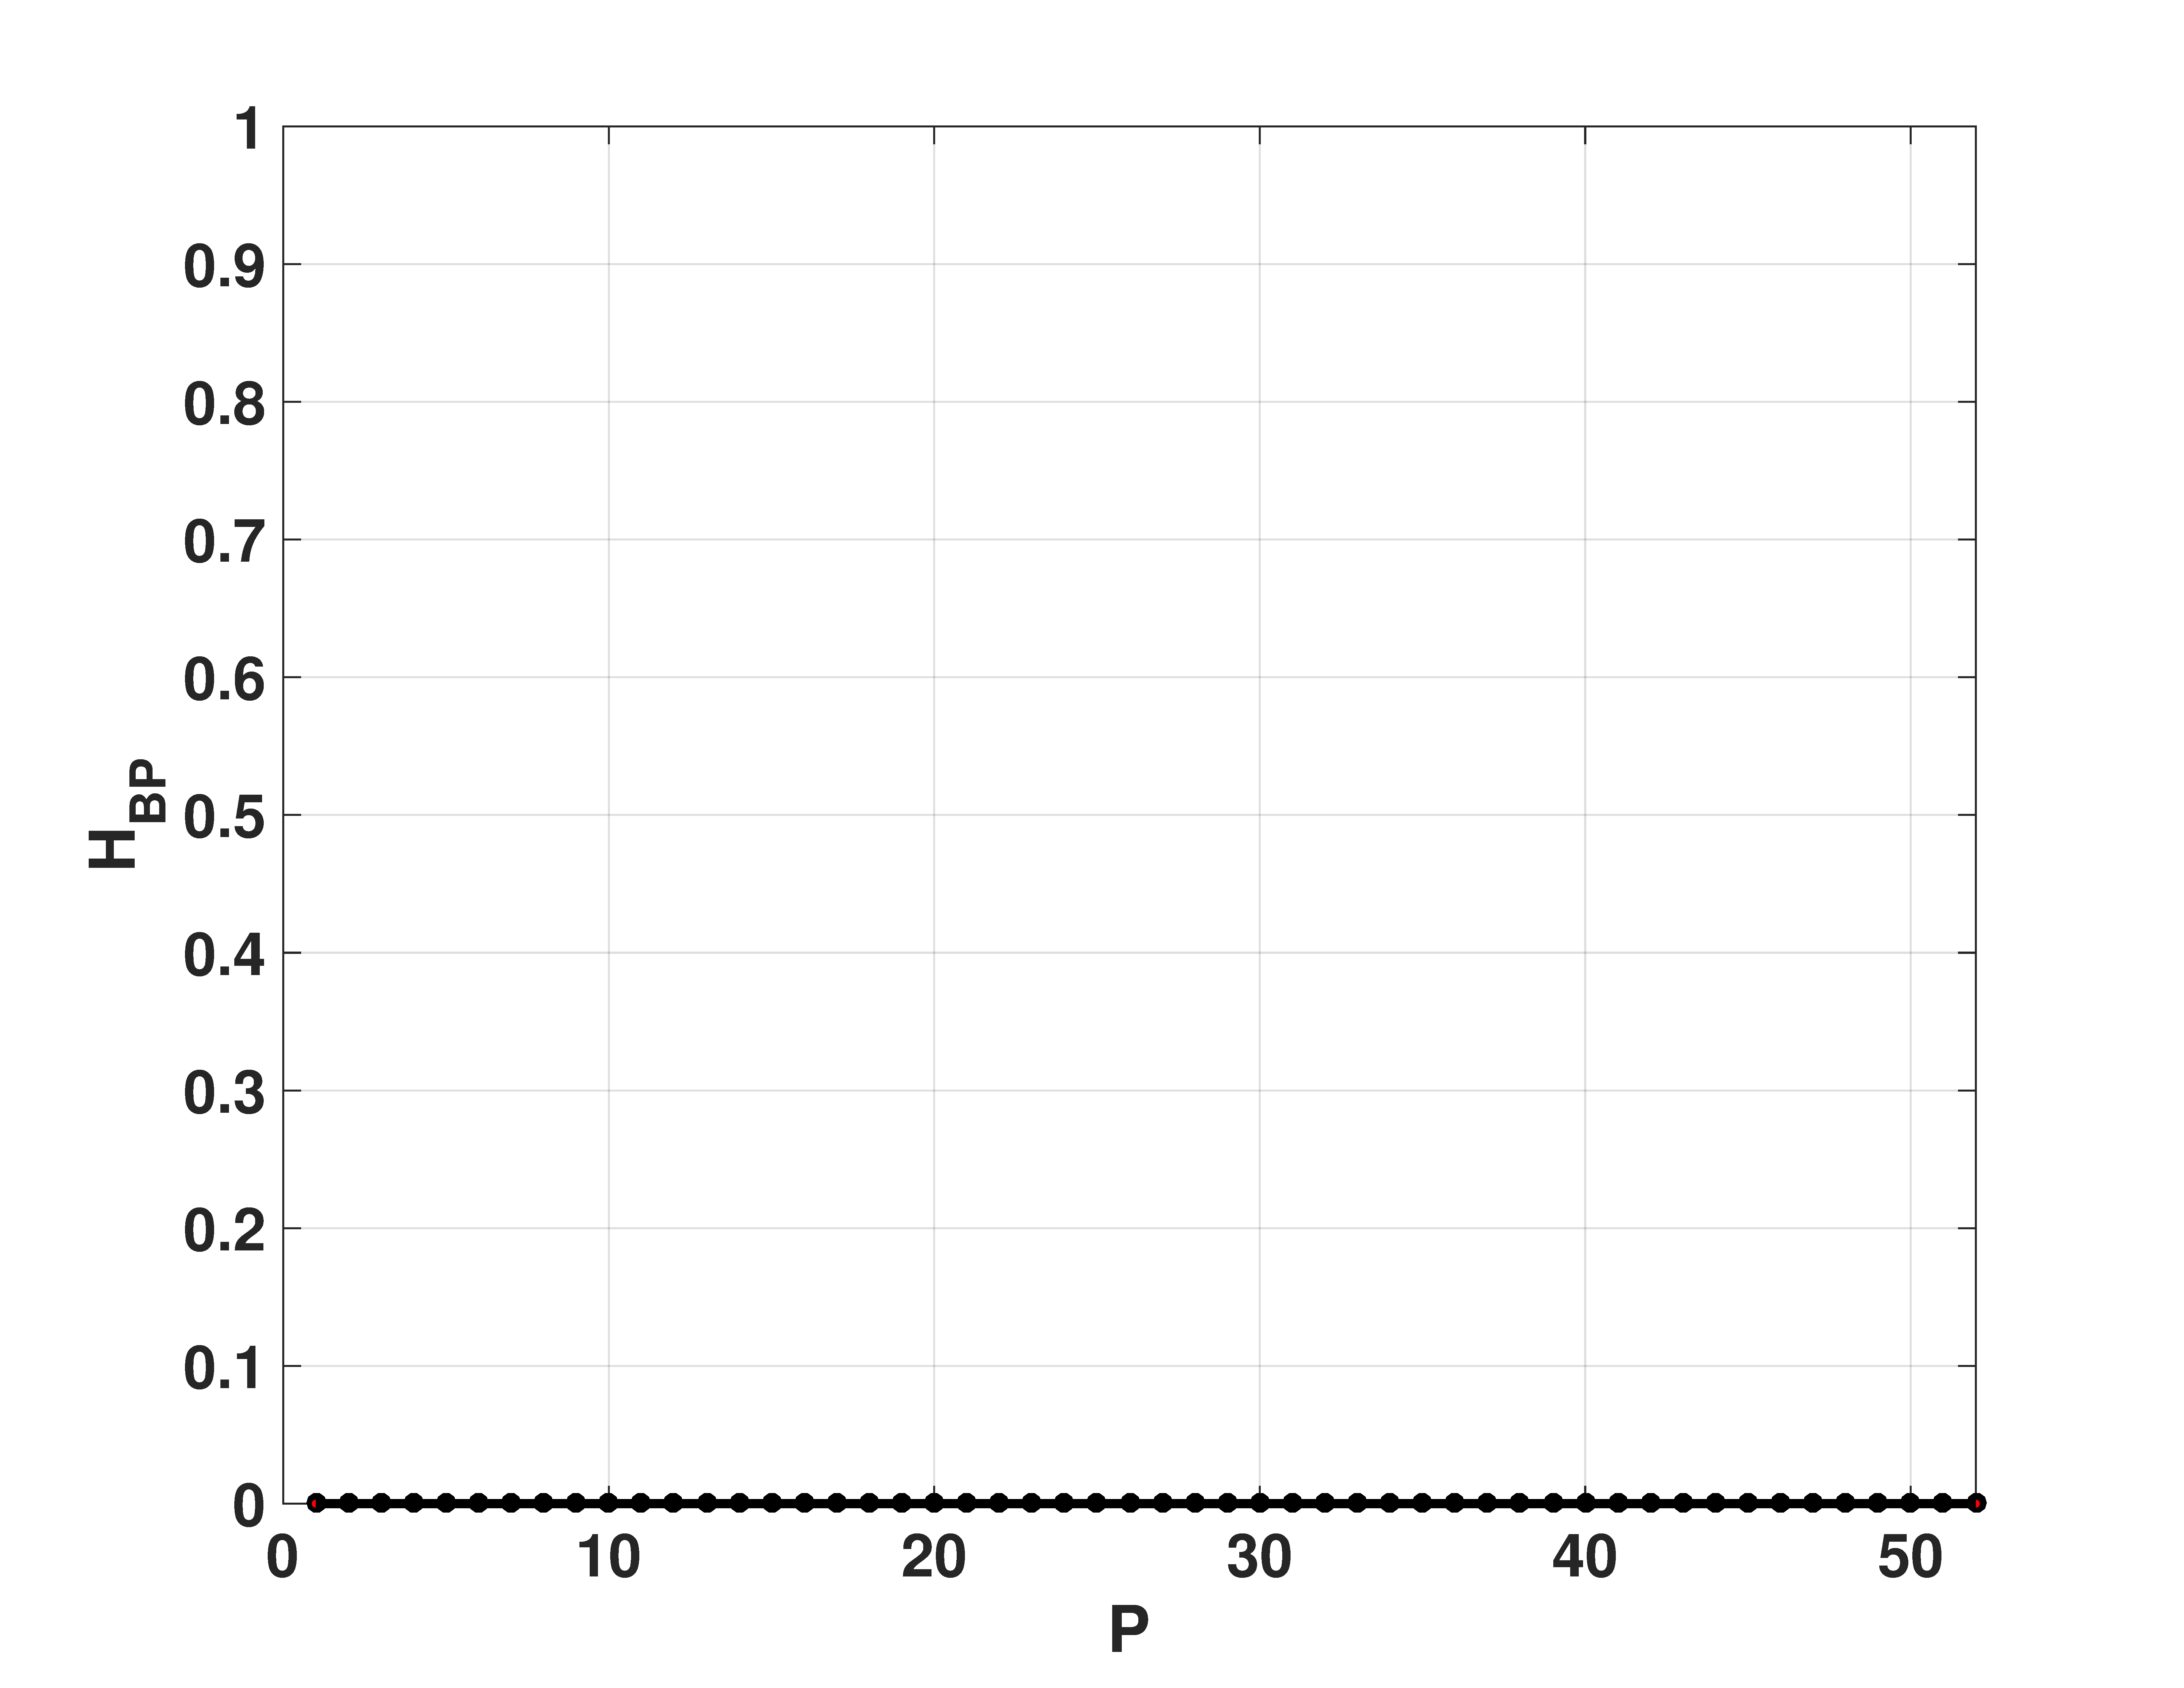
\includegraphics[width=.49\textwidth]{Hbp_Tent}
	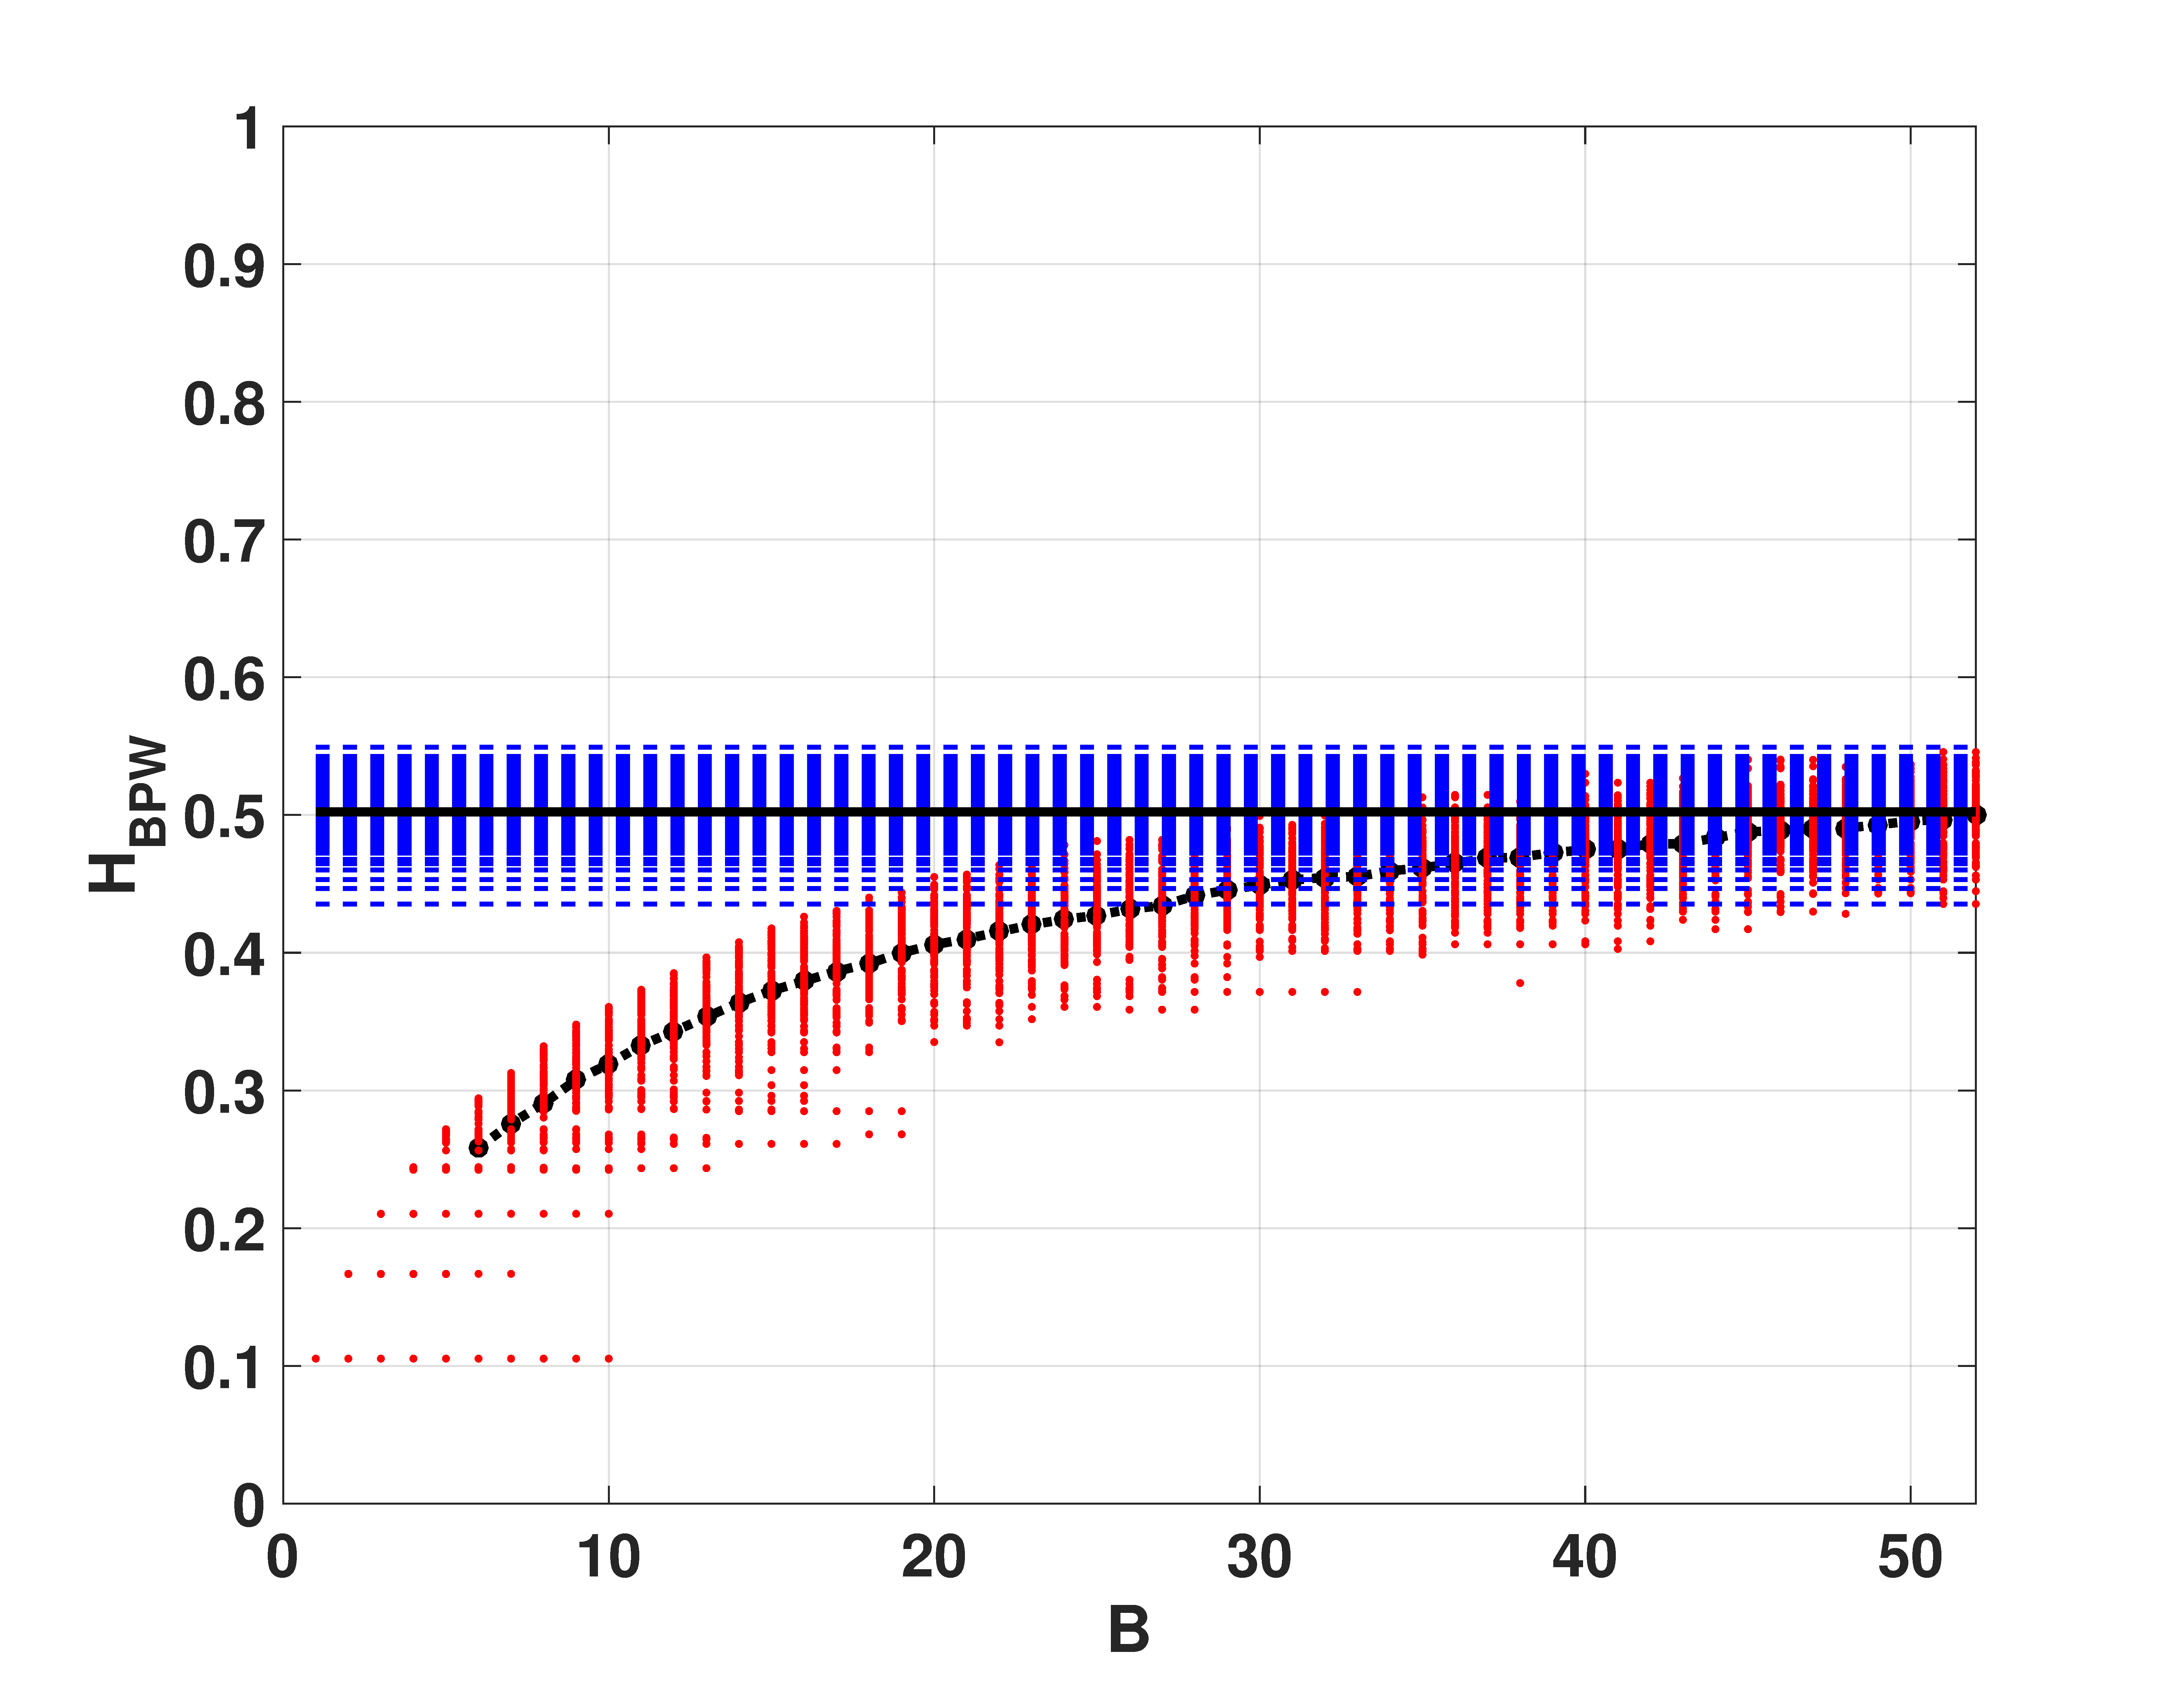
\includegraphics[width=.49\textwidth]{Hbpw_Tent}
	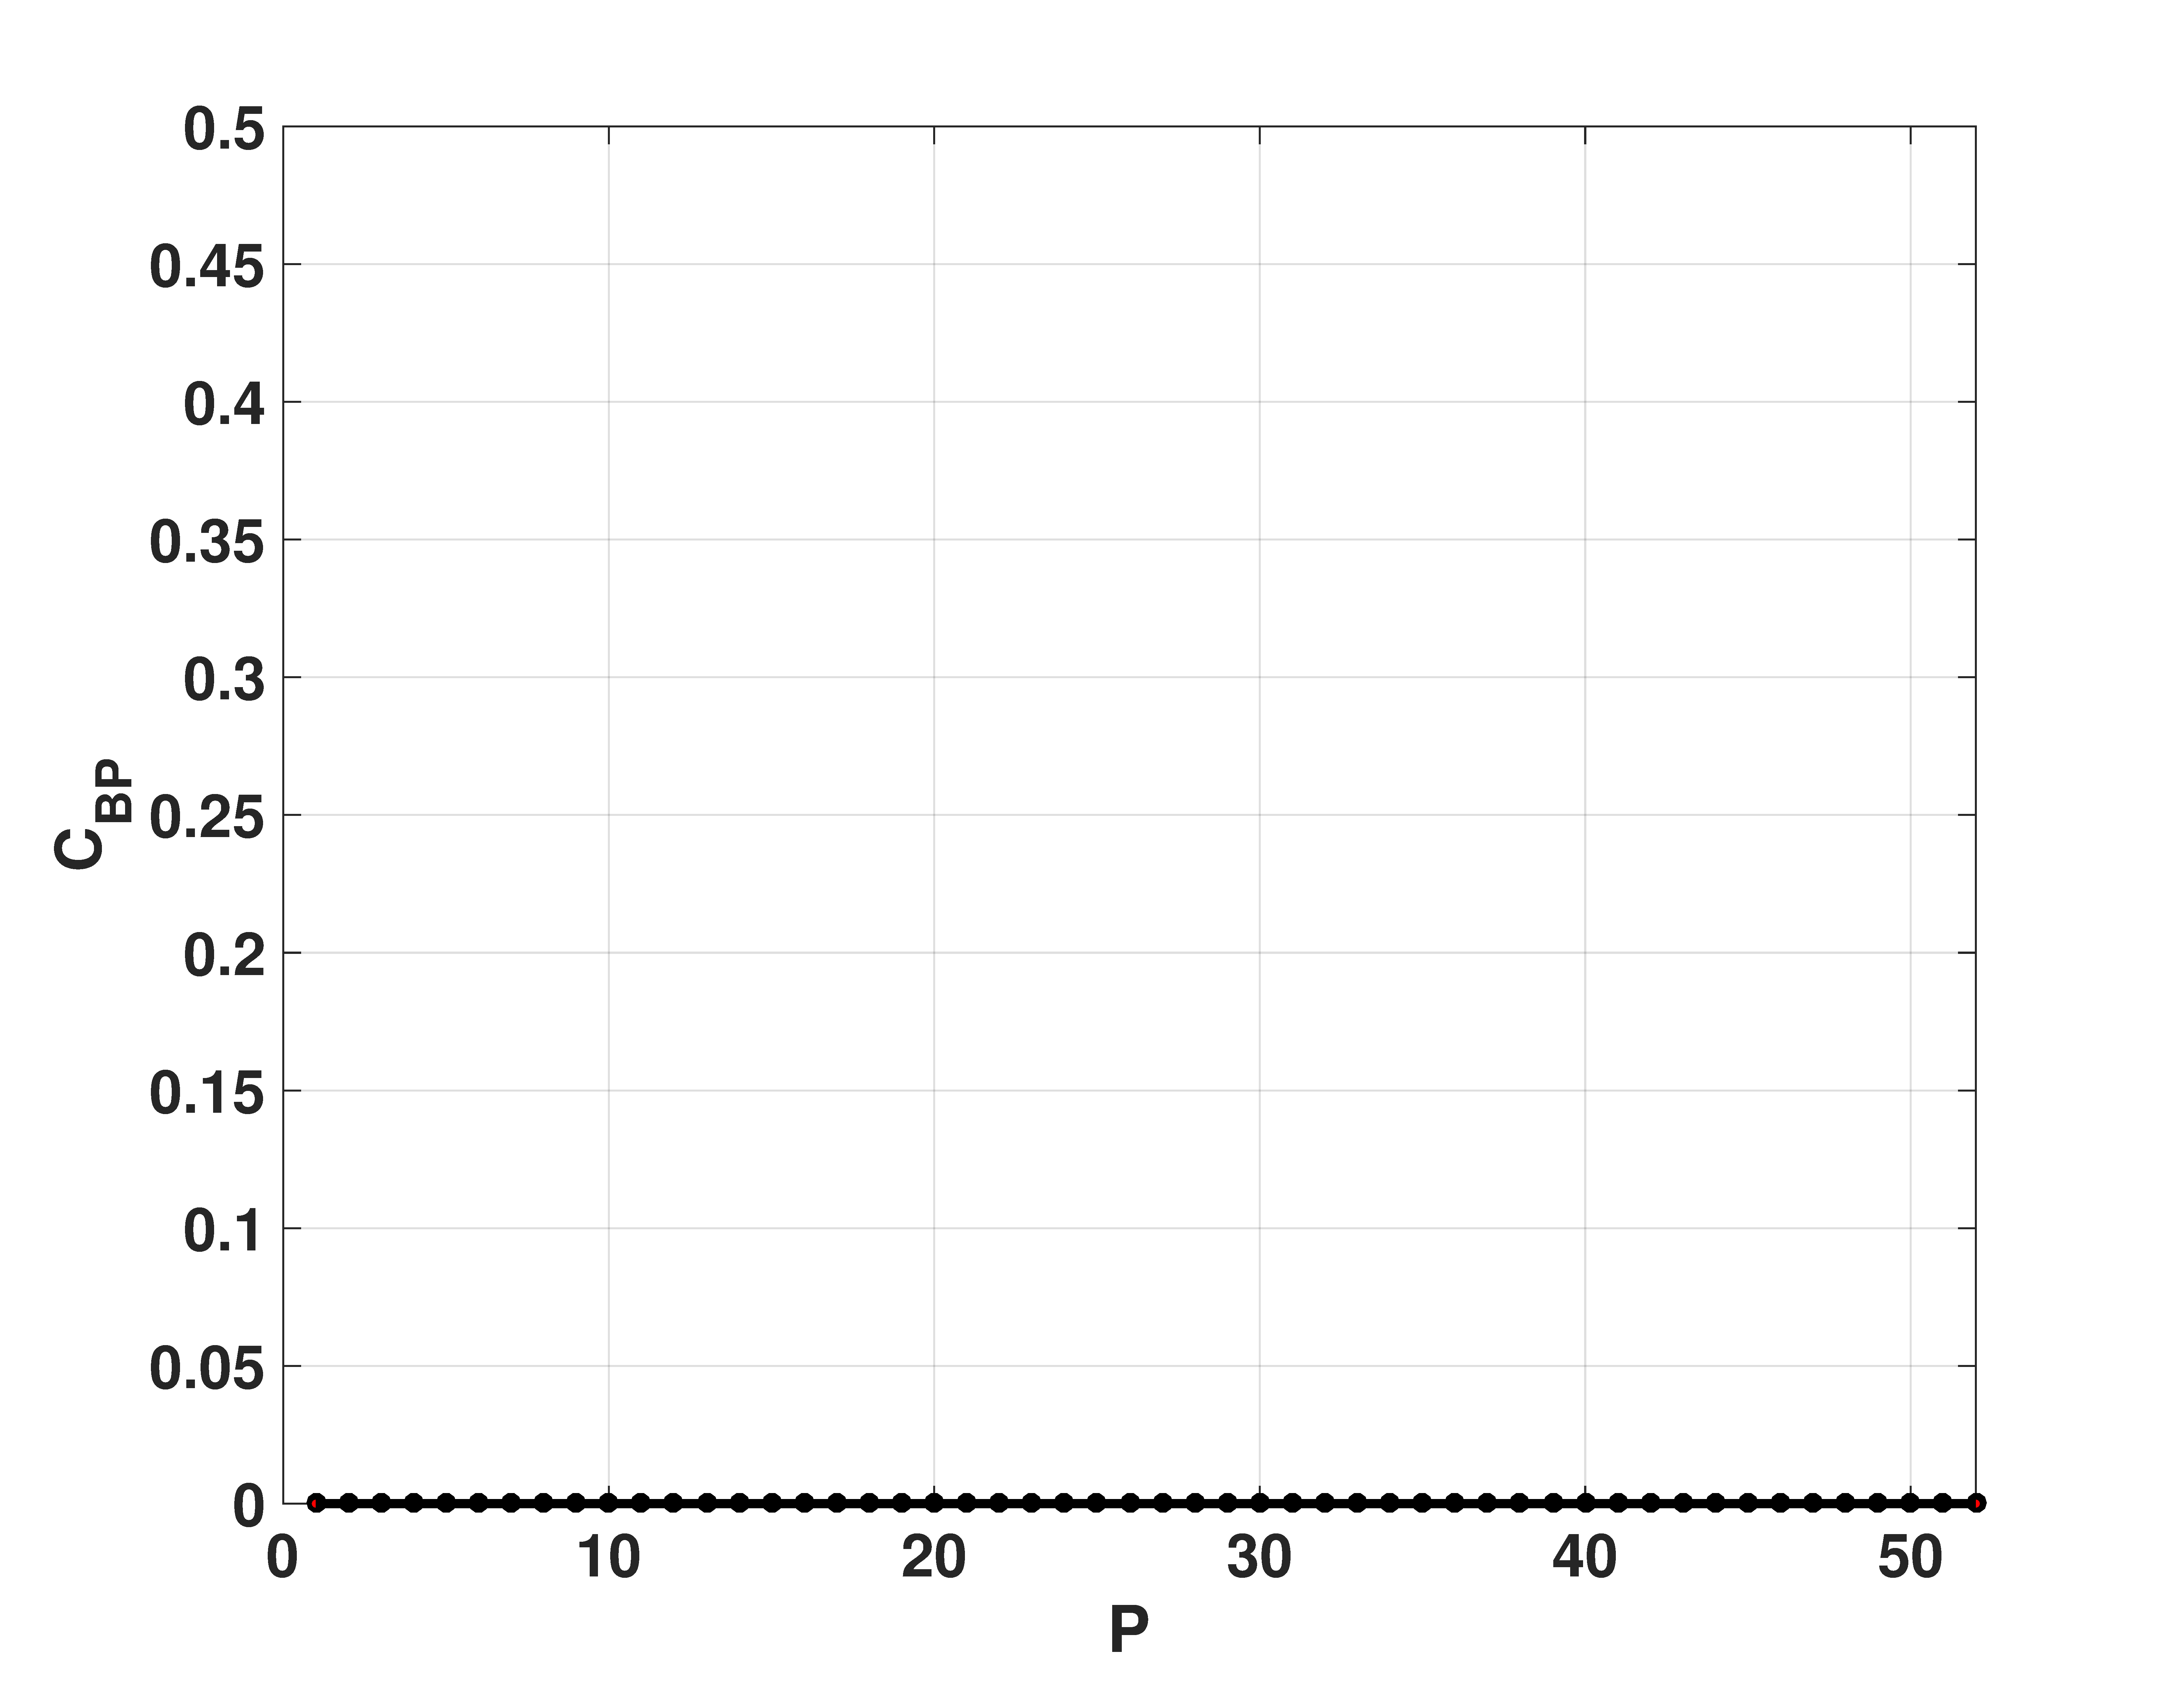
\includegraphics[width=.49\textwidth]{Cbp_Tent}
	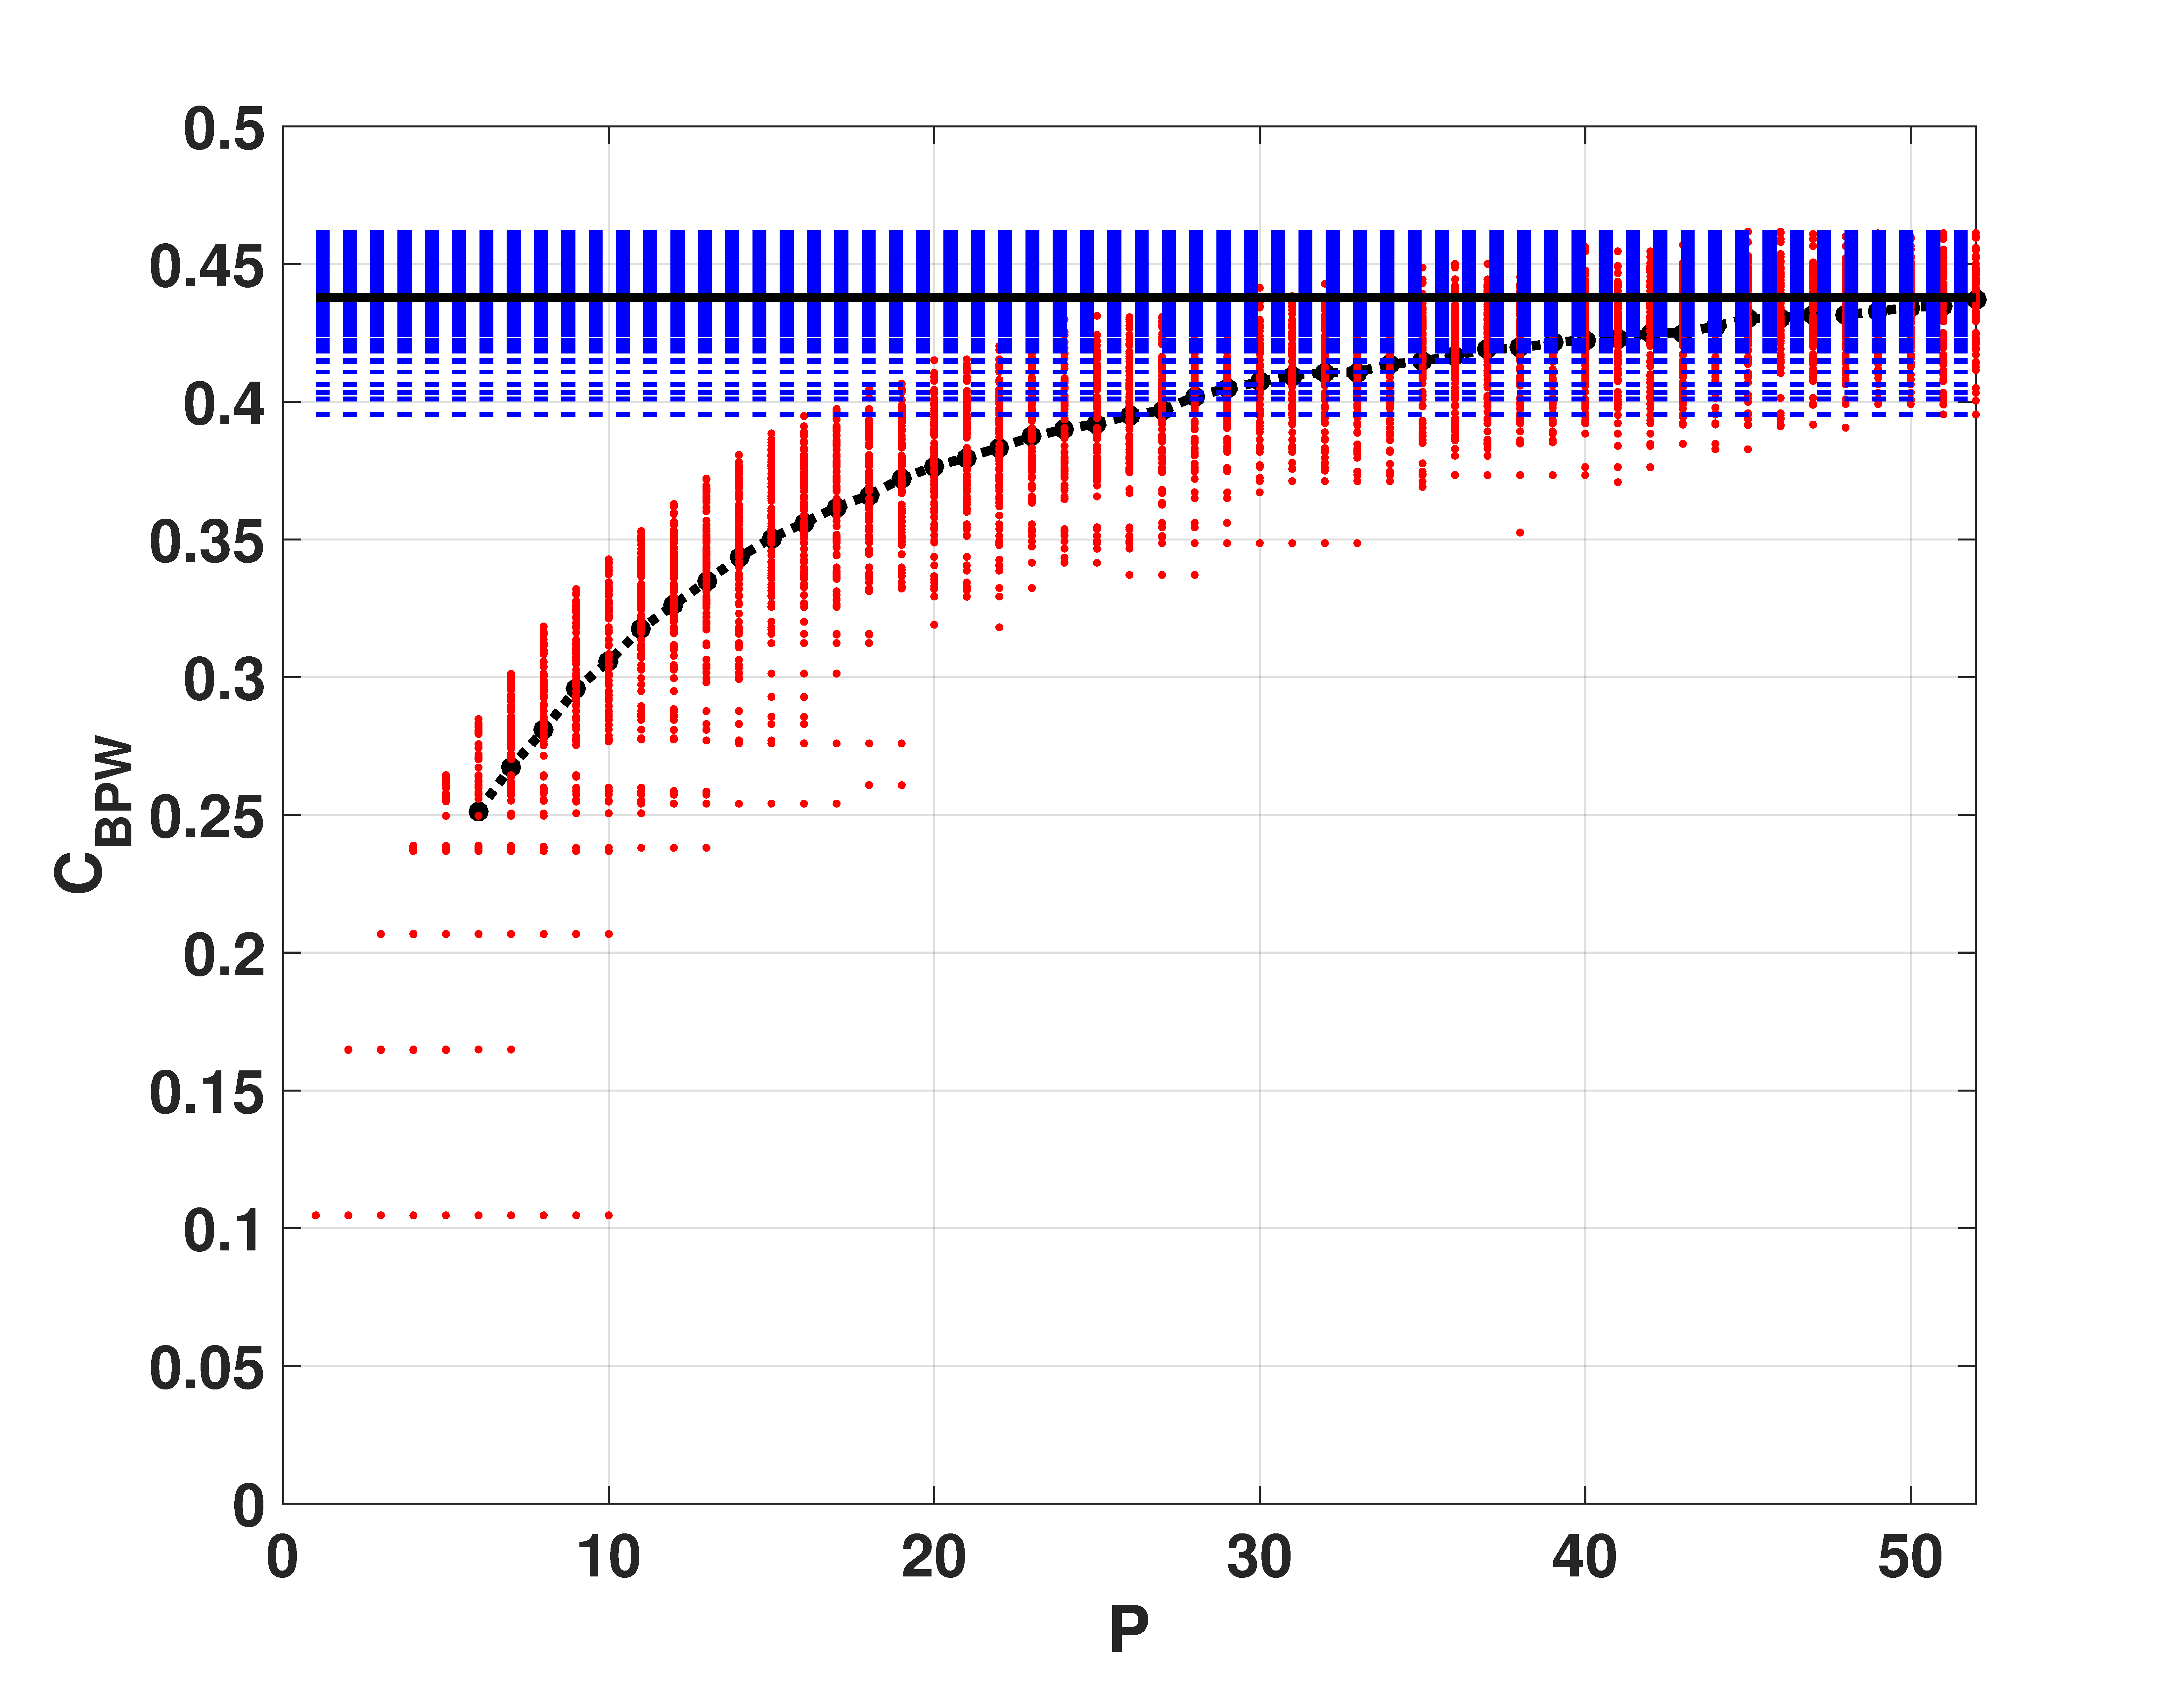
\includegraphics[width=.49\textwidth]{Cbpw_Tent}
	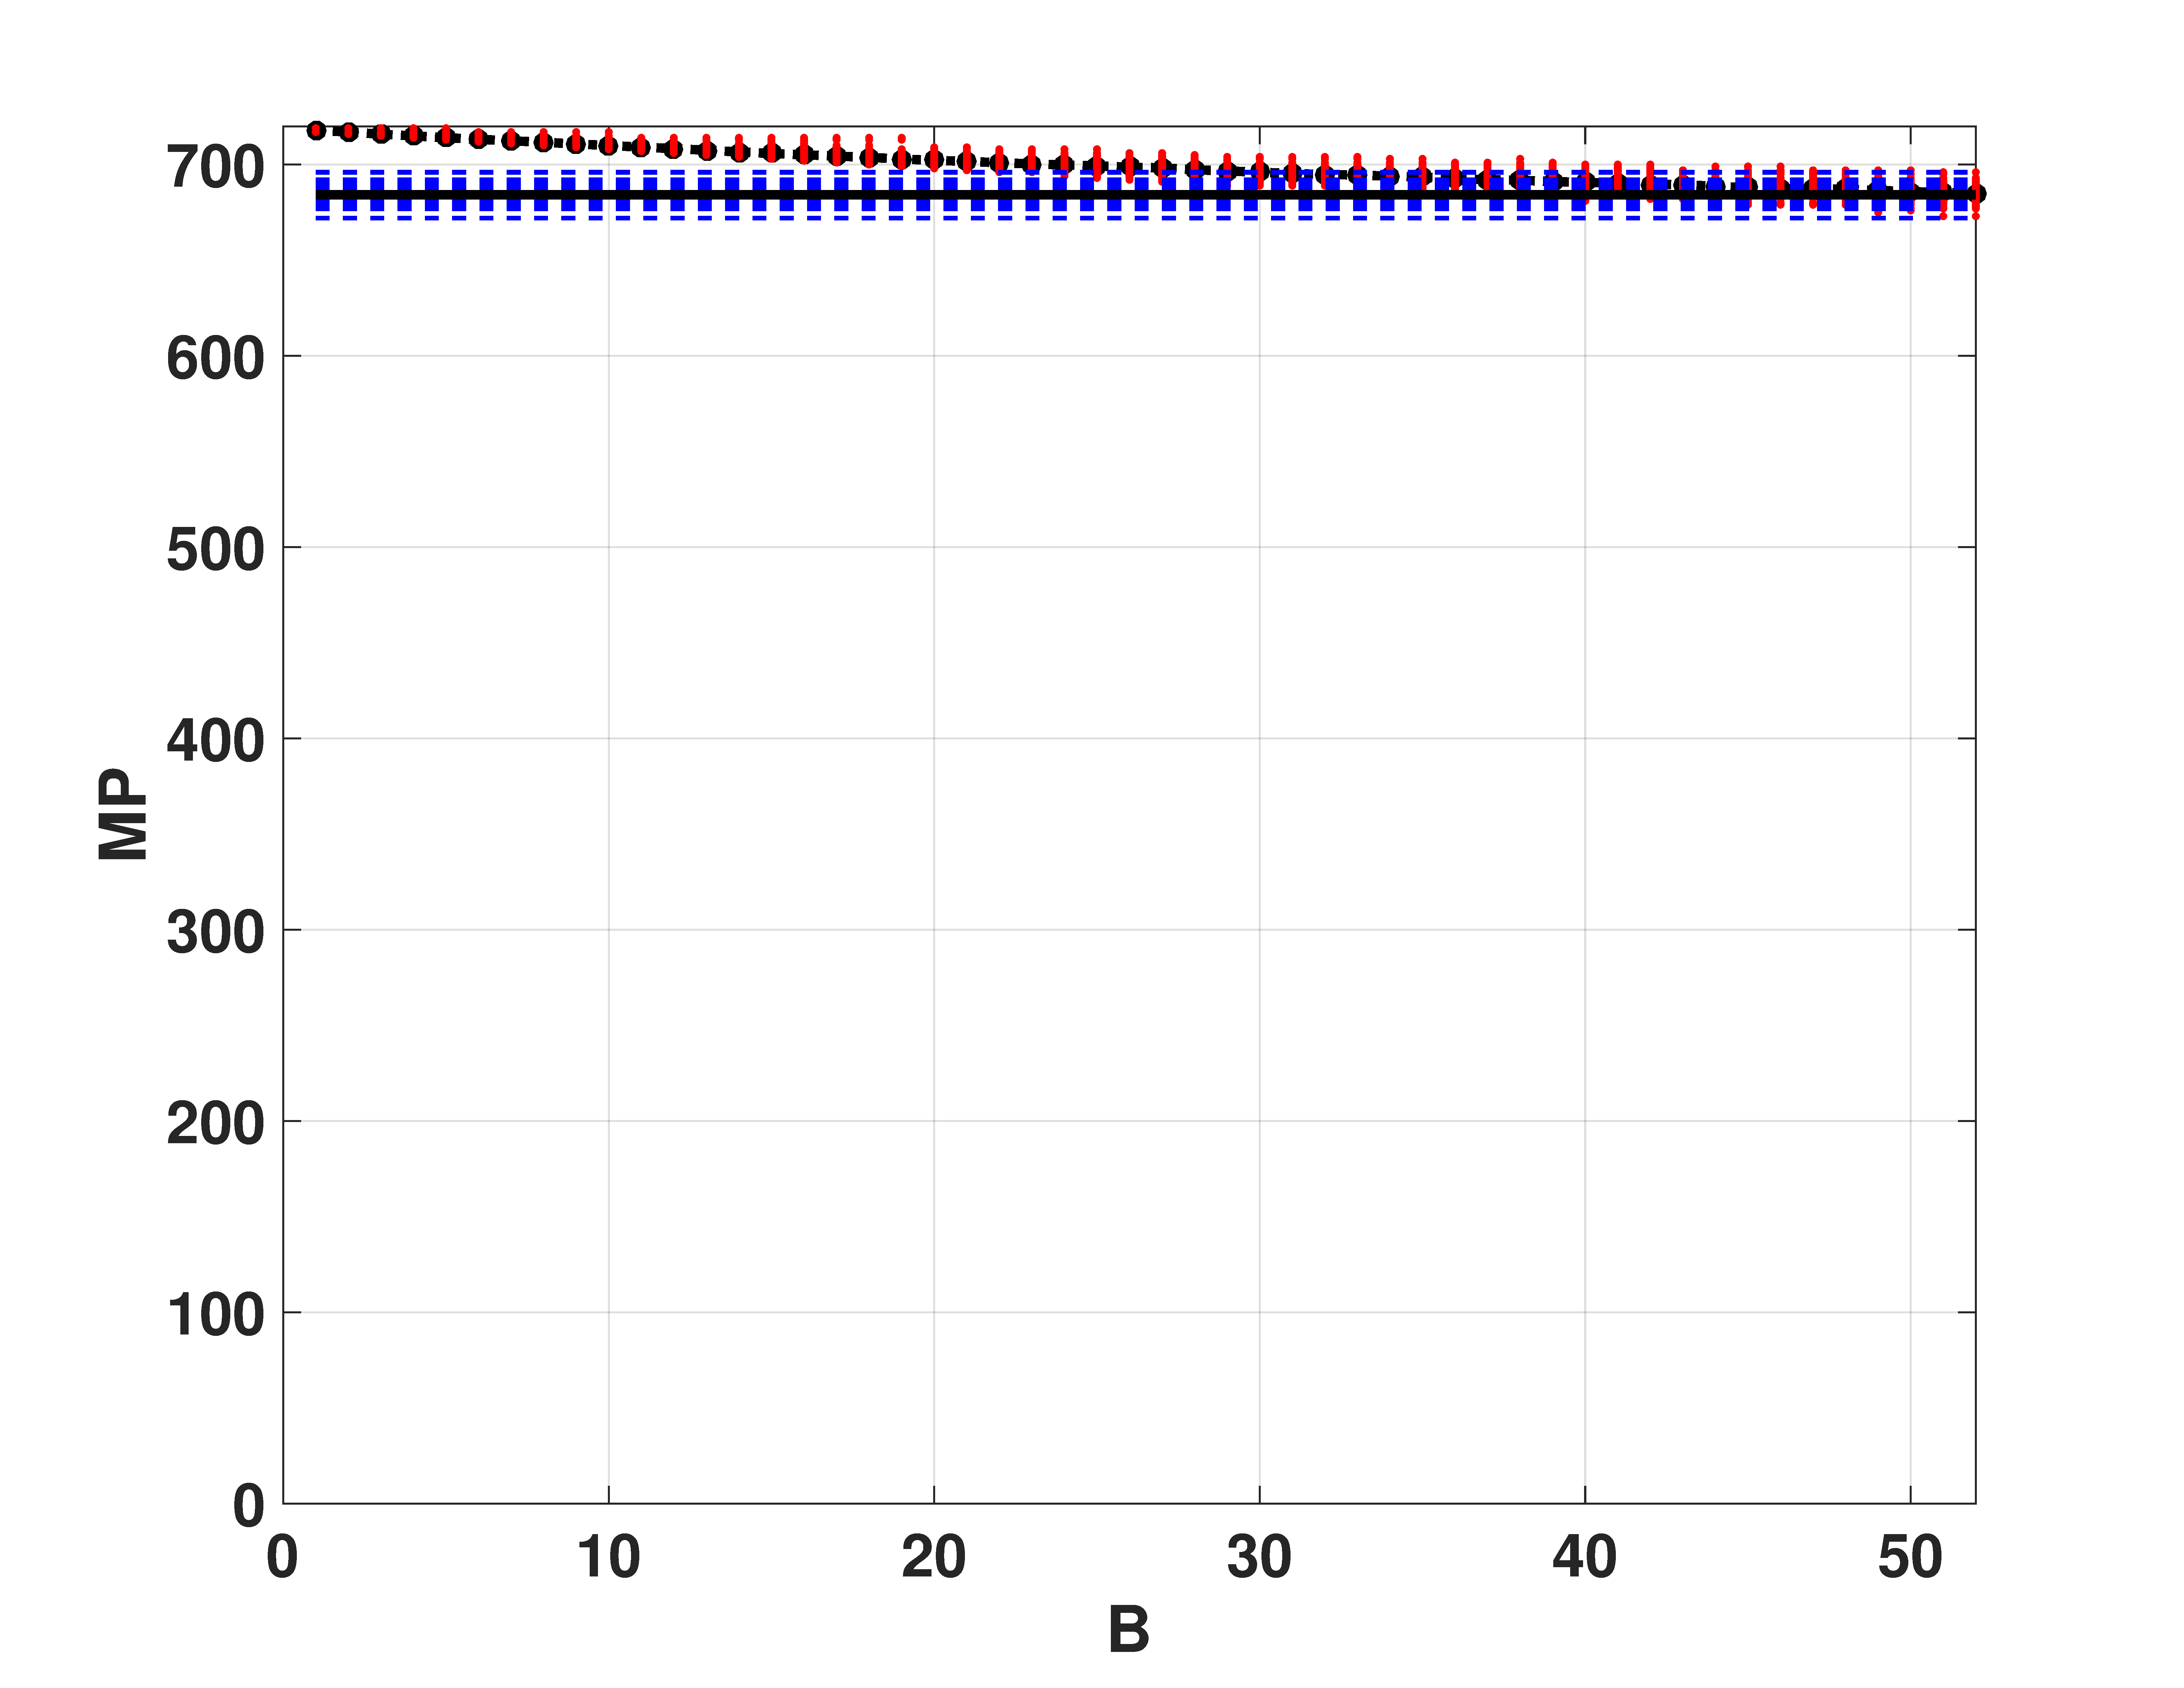
\includegraphics[width=.49\textwidth]{MP_Tent}
	\caption{Statistical properties of the TENT map: (a) $H_{hist}$ vs $B$ (b) $H_{BP}$ vs $B$ (c) $C_{BP}$ vs $B$ (d) $MP$ vs $B$.}
	\label{fig:TENT_QuantiB}
\end{figure}

Summarizing, in spite of using a high number of bits (with any 2-based numerical representation) to represent the digitalized TENT map it always loses the chaotic behaviour.
